 
% -*- root: ../../main.tex -*-
\section{ECS}
\label{sec:ecs_design}
Tradizionalmente nello sviluppo di applicazioni si tende ad utilizzare un approccio di design basato sull'\textbf{ereditarietà}. Questa scelta, attraverso la crea-zione di \textbf{gerarchie semantiche} precise (Persona -> Studente), permette generalmente di ottenere implementazioni più \textbf{robuste} e \textbf{strutturate}. Nell'ambito dei videogiochi, dove è necessario un elevato grado di \textbf{flessibilità}, queste gerarchie strutturate possono risultare \textbf{costrettive}.
Al fine di eliminare questa problematica nel tempo ci si è diretti verso approcci basati maggiormente sulla \textbf{composizione}. Il pattern architetturale \texttt{ECS} nasce proprio seguendo questa filosofia di pensiero.

\subsection{Il Pattern}
\label{subsec:ecs_pattern}
Il modello \textbf{ECS} è costituito da tre parti fondamentali: entità, componenti e sistemi.
\begin{itemize}
	\item{\textbf{Entity:}} costituisce una \textbf{rappresentazione astratta} di una entità in gioco. Essa è caratterizzata in un dato momento da una serie di proprietà che possono \textit{variare liberamente}. \textit{Concettualmente}, pur avendo un aspetto \textbf{dinamico} dal punto di vista delle proprietà ad essa associate, un'entità deve rimanere \textbf{fedele} alla sua natura. 

	Per esempio un'entità nemica manterrà sempre la sua natura avversa al giocatore, pur avendo la possibilità di \textit{modificare le sue proprietà}.
	\item{\textbf{Component:}} le proprietà associate all'entità prendono il nome di \textbf{componenti}. Essi sono la vera \textbf{componente modulare} di ECS poiché possono essere \textbf{aggregati} ad ogni entità in modo \textbf{dinamico}. La loro composizione costituisce lo \textbf{stato} dell'entità a cui sono associati.
	\item{\textbf{System:}} il sistema rappresenta il vero aspetto \textbf{funzionale} di ECS poiché costituisce un \textit{modulo} dedicato unicamente alla gestione del \textbf{comportamento} delle singole entità. Il punto di forza del pattern sta nel fatto che ogni \textbf{sistema agisce} su una serie di \textbf{componenti} (in base alla tipologia), di conseguenza nel momento in cui un componente verrà rimosso da un'entità quest'ultima vedrà \textbf{modificato} il proprio comportamento.
\end{itemize}

\subsection{Approcci di Design}
Come visto in precedenza in \ref{subsec:ecs_pattern}, l'idea alla base di ECS è molto semplice, tuttavia durante il processo di \textbf{concretizzazione} alcuni aspetti concettuali vengono realizzati in modo leggermente diverso per \textit{esigenze di carattere implementativo} (performance, cache, ecc).  Dal punto di vista progettuale esistono diversi \textbf{approcci possibili}:
\begin{itemize}
	\item{\textbf{Approccio OOP:}} questa tipologia di approccio riprende l'idea che sta alla base della \textbf{programmazione ad oggetti}; in particolare viene promosso il concetto secondo il quale ogni oggetto possiede al proprio interno uno \textbf{stato} e un \textbf{comportamento}. Un ECS di tipo OOP sarà caratterizzato da entità che \textbf{contengono} i propri \textbf{componenti} e si occupano della loro \textbf{gestione}.
	\item{\textbf{Approccio Funzionale:}} in questo caso stato e comportamento vengono mantenuti in \textbf{moduli dedicati} promuovendo una maggiore \textbf{separazione dei concetti}. L'ECS in questo caso sarà caratterizzato da \textbf{moduli di gestione} ai quali sarà delegata il \textbf{controllo} e la \textbf{connessione} di entità e componenti.
\end{itemize}

\begin{figure}[H]
	\centering
	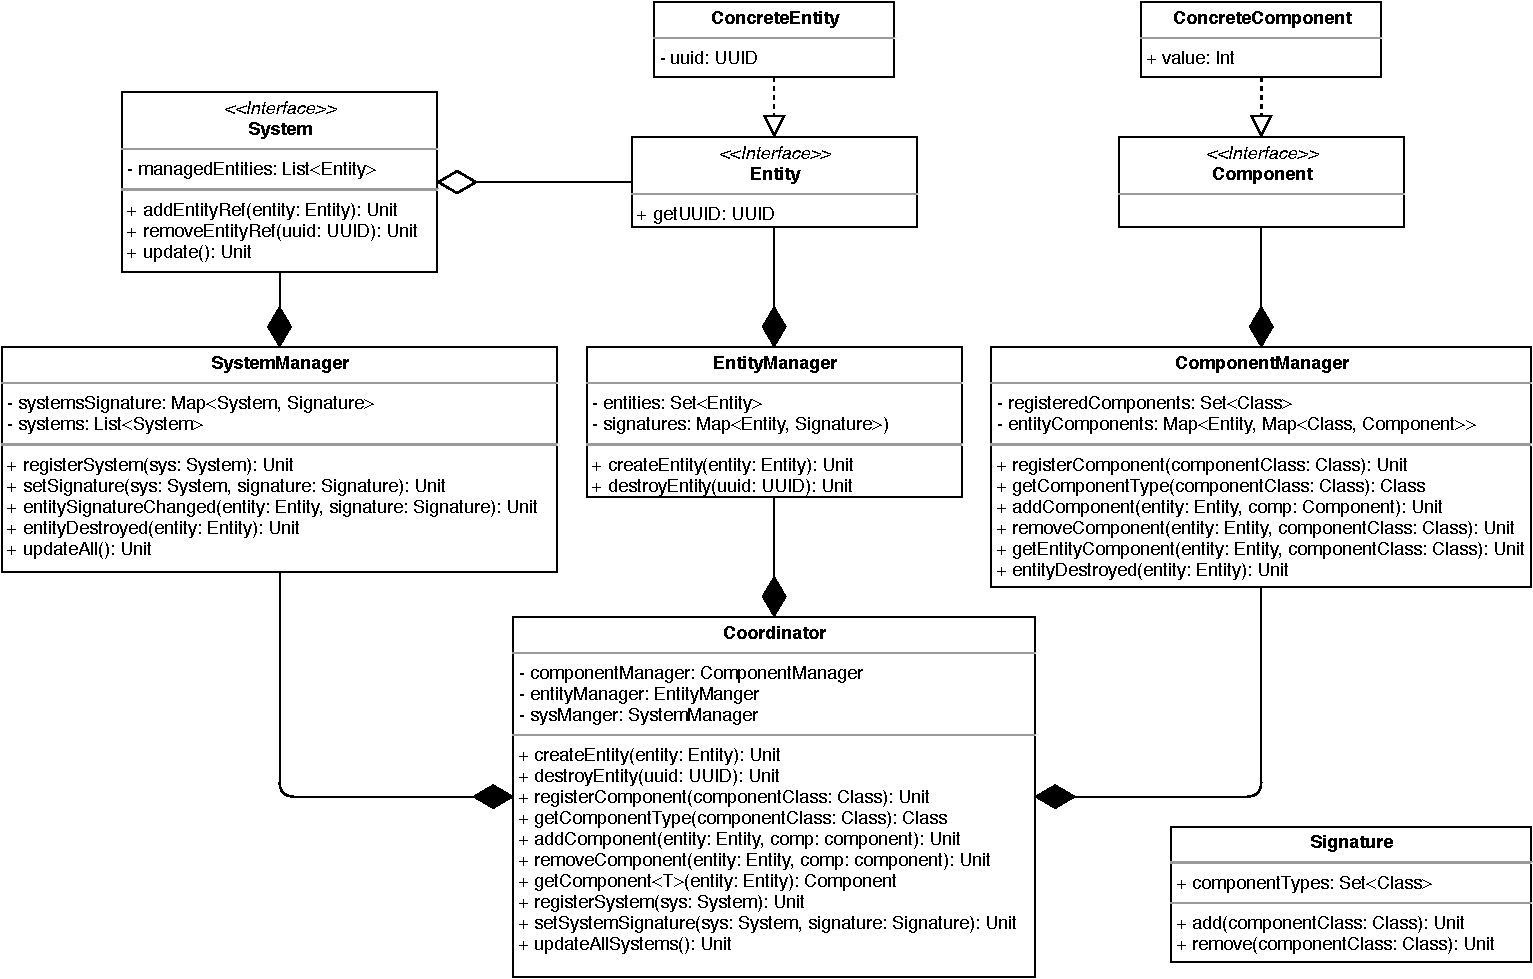
\includegraphics[width=0.99\columnwidth]{drawio/ECS/ECS.pdf}
	\caption{}
	\label{fig:ECS}
\end{figure}


% section section_name (end)
 %giustificazione ecs
 %Ogni sistema si occupa di gestire solamente uno o più componenti, aggiornandoli in blocco contemporaneamente. Questo approccio, in contrasto con l'approccio più OOP che consisterebbe nel modellare ogni entità come un oggetto, che deve implementare una sotto-interfaccia diversa in base al tipo, ereditando i metodi per l'aggiornamento. Questo causa problemi di performance all'aumentare delle entità da gestire, infatti ad ogni aggiornamento sarà caricato in cache l'intero oggetto e andrà recuperato dalla virtual table(TODO CHECK THIS) il metodo relativo all'aggiornamento. Ciò comporta un degradamento importante delle performance dato che gli accessi in RAM sono molto più lenti di quelli direttamente in cache. Sfruttando l'approccio ECS invece è possibile sfruttare meglio la cache, in quanto per ogni aggiornamento i componenti vengono caricati cache in blocco e processati dallo stesso metodo. 
	\subsubsection{Interazione tra Engine, ECS e controller}
	 
	Come spiegato nel \ref{sec:ecs_design}, i vari gestori di componenti che compongono l'ECS sono coordinati tra di loro tramite un coordinator. Esso fa da punto di contatto con l'engine vero e proprio esponendo il metodo \emph{updateAllSystems}, che corrisponde a un tick del gioco. Esso viene incapsulato nel metodo \emph{update} esposto dall' interfaccia \textbf{UpdateableEngine}, implementata dal \emph{GameEngine}. In questo modo è possibile per il \emph{GameLoop} interagire con l'engine.
	Quando il gioco è fatto eseguire in modalità singleplayer il controller si occupa di creare l'engine e al join di una partita multiplayer esso verrà deallocato e verrà creato l'attore client.
	\begin{figure}[H]
		\centering
		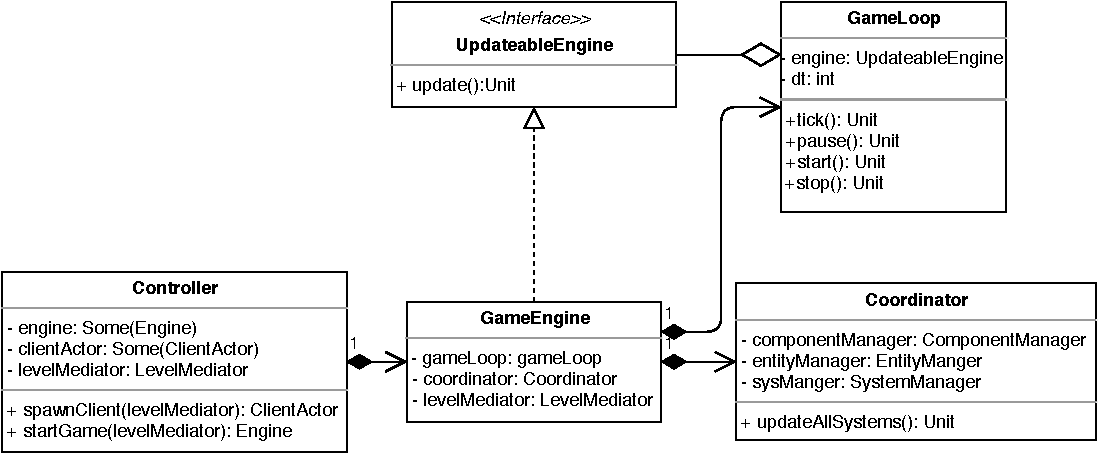
\includegraphics[width=\columnwidth]{drawio/ECS-engine-controller/ecs-engine-controller.pdf}
		\caption{Diagramma raffigurante ecs, engine e controller e le loro interazioni.}
		\label{fig:ecsenginecontroller}
	\end{figure}